%% Based on a TeXnicCenter-Template by Gyorgy SZEIDL.
%%%%%%%%%%%%%%%%%%%%%%%%%%%%%%%%%%%%%%%%%%%%%%%%%%%%%%%%%%%%%


%------------------------------------------------------------
%
%\documentclass{article}
%\documentclass[twocolumn]{article}%
\documentclass[11pt,onecolumn]{article}
%\documentclass[10pt,letterpaper, titlepage]{article}
%\documentclass{proc}
%Options -- Point size:  10pt (default), 11pt, 12pt
%        -- Paper size:  letterpaper (default), a4paper, a5paper, b5paper
%                        legalpaper, executivepaper
%        -- Orientation  (portrait is the default)
%                        landscape
%        -- Print size:  oneside (default), twoside
%        -- Quality      final(default), draft
%        -- Title page   notitlepage
%        -- Columns      twocolumn
%        -- Equation numbering (equation numbers on the right is the default)
%                        leqno
%        -- Displayed equations (centered is the default)
%                        fleqn (equations start at the same distance from the right side)
%        -- Open bibliography style (closed is the default)
%                        openbib
% For instance the command
%           \documentclass[a4paper,12pt,leqno]{article}
% ensures that the paper size is a4, the fonts are typeset at the size 12p
% and the equation numbers are on the left side
%
%\documentclass[a4paper,12pt,leqno]{article}

%\usepackage{amsmath}%
%\usepackage{amsfonts}%
%\usepackage{amssymb}%
%\usepackage[latin1]{inputenc} %Codificaci�n europea del teclado
\usepackage[T1]{fontenc} %Dispone de fuentes tipos car�cteres acentuados
\usepackage[spanish]{babel} 
\usepackage{babelbib}
%\usepackage[annote,languagenames,fixlanguage]{babelbib}
%\setbtxfallbacklanguage{spanish}
\usepackage[lmargin=2cm,rmargin=2.5cm,tmargin=3cm,bmargin=2cm]{geometry}
\usepackage{amsfonts}
\usepackage{graphicx}

\title{Planificaci\'on Preoperatoria Digital en Traumatolog\'ia}

\author{Esmitt Ram\'irez Jacobo}
\date{Abril 2009}
%%
%%\hyphenation{pro-ce-di-miento pro-ce-di-mientos pre-ope-ra-to-ria mo-da-li-da-des dia-fi-sia-rias rea-li-cen %%pla-ni-fi-ca-cion or-ga-nis-mo he-rra-mien-ta co-rres-pon-diente exis-te par-ti-cu-lar-mente li-te-ra-tu-ra i-ma-ging %%bi-blio-graf-fi-ca }

%\marginsize{1cm}{1cm}{1cm}{1cm}
%\topmargin{1pt}
%\setlength{\leftmargin}{-5.0in}
%%%%%%%%
%% tipo de numeracion
%\pagenumbering{alph}
%%%%%%%%
%\pagestyle{plain}
%\pagestyle{empty}
%\pagestyle{headings}
\pagestyle{myheadings}
\markboth{Planificaci\'on Preoperatoria Digital en Traumatolog\'ia}{E. RAMIREZ}
%\markright{Planificaci\'on Preoperatoria Digital en Traumatolog\'ia}
%\markright{aaaa}

\begin{document}
\maketitle

%%%%%%%%%%%%%%%%%%%%%%%%%%%%%%%%%%%%%%%%%%%
\begin{abstract}
En este documento se presenta un esquema para la planificaci\'on preoperatoria digital en el \'area de Traumatolog\'ia. La planificaci\'on preoperatoria consta de una serie de procedimientos previos a una operaci\'on que el cirujano ortopedista debe realizar para garantizar la eficacia de la misma. Dichos procedimientos requieren de material adicional (papel, l\'apiz, regla, etc.) y una inversi\'on de tiempo considerable para su realizaci\'on. Una soluci\'on es emplear un sistema CAD de planificaci\'on preoperatoria  para fracturas de huesos, tal que sea una simplificaci\'on en su elaboraci\'on. Se presenta entonces una explicaci\'on del proceso completo de planificaci\'on preoperatoria as\'i como de una revisi\'on bibliogr\'afica sobre los trabajos realizados en este sentido, finalmente se propone un esquema que deben seguir los sistemas de planificaci\'on preoperatoria.
\end{abstract}

%%%%%%%%%%%%%%%%%%%%%%%%%%%%%%%%%%%%%%%%%%%
%\begin{keywords} Traumatolog\'ia, Sistemas CAOS, Planificaci\'on Preoperatoria.
%\end{keywords}

%\pagestyle{myheadings}%PONE LA NUMERACION A LA DERECHA
%\thispagestyle{plain}
%\markboth{E. RAM\'IREZ}{Planificaci\'on Preoperatoria Digital en Traumatolog\'ia}
%\markboth{E. RAM\'IREZ}{Planificaci}
%\markboth{left head}{right head}

%\markright{right head} 

%%%%%%%%%%%%%%%%%%%%%%%%%%%%%%%%%%%%%%%
%%%%%%%%%%%%%%%%%%%%%%%%%%%%%%%%%%%%%%%
\section{Introducci\'on}

Desde que Wilhelm R\"oentgen \cite{HOLL90} descubriera la existencia de los Rayos-X en 1895, las im\'agenes m\'edicas han tenido un gran avance dentro de la Medicina, dando origen a t\'ecnicas como: fluoroscop\'ia, US (\textit{Ultrasound} - Ultrasonido), CT (\textit{Computed Tomography} - Tomograf\'ia Computarizada), MRI (\textit{Magnetic Resonance Imaging} - Imagen por Resonancia Magn\'etica) entre otras. Todas estas modalidades de im\'agenes constituyen una base fundamental para los diagn\'osticos m\'edicos dentro de los sistemas de salud modernos a nivel mundial.

Los progresos en tecnolog\'ia de tratamiento digital de im\'agenes est\'an regidos en parte por la velocidad en la que avanzan los desarrollos e investigaciones en el \'area de la Computaci\'on. Los sistemas CAD (\textit{Computer Aided Diagnosis} - Dise\~no Asistido por Computador) fueron surgiendo como herramientas de apoyo a los m\'edicos en la toma de decisiones. Es indudable que el progreso de los sistemas CAD dentro del \'area m\'edica viene dado en la misma proporci\'on que exista ese progreso tecnol\'ogico dentro de la medicina.

Dentro de los sistemas CAD, existe una clasificaci\'on conocida como sistemas CAOS (\textit{Computer Aided Orthopaedic Surgery} - Cirug\'ia Ortop\'edica Asistida por Computador), los cuales permiten asistir al cirujano ortop\'edico en la planificaci\'on preoperatoria de cirug\'ias del sistema muscoesquel\'etico. La planificaci\'on preoperatoria es el primer paso en el manejo del paciente que va a ser sometido a una cirug\'ia ortop\'edica, puesto que permite establecer la t\'actica quir\'urgica en el procedimiento a realizar, siendo adem\'as una gu\'ia fidedigna para determinar el resultado final de la cirug\'ia; sin embargo este procedimiento puede ser realizado de manera imprecisa y poco efectiva.

Solo algunos cirujanos ortop\'edicos llevan a cabo dichas planificaciones, por el requerimiento de material adicional y la inversi\'on considerable de tiempo para su realizaci\'on. Los sistemas CAOS son excelentes herramientas para que los m\'edicos realicen dicha planificaci\'on en un tiempo m\'as corto y una menor cantidad de materiales. Cada vez es m\'as frecuente la presencia de estos sistemas en el campo de la medicina, particularmente existe un gran crecimiento en el \'area de Radiolog\'ia \cite{GIGE00}.

En este documento, se explica en detalle los aspectos relacionado con la planificaci\'on preoperatoria presentando un esquema para los sistemas CAOS tal que realicen las planificaciones prequir\'urgicas digitales de fracturas diafisiarias. Al mismo tiempo, el esquema planteado permite el almacenamiento de la informaci\'on obtenida para su posterior utilizaci\'on con fines de consulta y creaci\'on de un historial de experiencias (i.e. casos cl\'inicos documentados).

%%%%%%%%%%%%%%%%%%%%%%%%%%%%%%%%%%%%%%%
%%%%%%%%%%%%%%%%%%%%%%%%%%%%%%%%%%%%%%%
\section{Planificaci\'on Preoperatoria} 

La planificaci\'on preoperatoria o planificaci\'on prequir\'urgica es una disciplina sumamente importante que debe ser realizada por todos los cirujanos ortop\'edicos como requisito indispensable para llevar a cabo un determinado procedimiento quir\'urgico con excelentes resultados.

\begin{quote}
\textit{
	El tiempo que el cirujano ortopedista dedique a efectuar una cuidadosa planificaci\'on preoperatoria tiene una importancia decisiva y a menudo determina el \'exito o fracaso de una operaci\'on \cite{SCHA98}
	}
\end{quote}

La planificaci\'on preoperatoria ortop\'edica, es un procedimiento indispensable que debe realizarse previo a la intervenci\'on quir\'urgica y cuyos objetivos son: determinar el resultado final de la cirug\'ia y establecer la t\'actica quir\'urgica a seguir en el procedimiento quir\'urgico \cite{RUEDI03}. Seg\'un los procedimientos sugeridos en \cite{HOLD03} \cite{MAST89}, la planificaci\'on preoperatoria para una cirug\'ia plantea la realizaci\'on de calcos preoperatorios, como se muestra en la Figura \ref{fig:planificacion}. Los calcos permiten entender la complejidad de la fractura, la forma de reducci\'on de la misma, la aplicaci\'on del principio biomec\'anico y la elecci\'on del implante necesario.

\begin{figure}[htb]
	\centering
	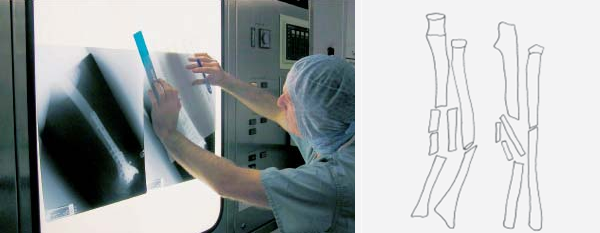
\includegraphics[width=.8\columnwidth]{images/planificacion_calco.png}
	\caption{(A)-Procedimiento para creaci\'on de un calco y (B)-el calco obtenido en la misma}
	\label{fig:planificacion}
\end{figure}

En ciertos procedimientos quir\'urgicos, la planificaci\'on preoperatoria es parte integral de una cirug\'ia. En la cirug\'ia para la colocaci\'on de una pr\'otesis de cadera \cite{EGGLI98} \cite{BENE03}, es importante conocer ciertos factores previos: tipo y tama\~no de pr\'otesis, posici\'on y orientaci\'on correcta de los implantes, tama\~no del acetabulo y del hueso; y as\'i reducir el tiempo de la cirug\'ia y obtener resultados satisfactorios.

Para tener \'exito en el resultado final de la cirug\'ia se deben de tomar en cuenta los factores iniciales del contacto m\'edico-paciente, realizar una historia completa, examen f\'isico detallado (incluyendo pruebas especiales), radiograf\'ias para la planificaci\'on de preferencia sin inmovilizadores que obstaculicen la visi\'on adecuada \cite{RUEDI03}, estudios especiales como CT, MRI, estudios de laboratorio completos, evaluaci\'on preoperatoria y la planificaci\'on preoperatoria.

%%%%%%%%%%%%%%%%%%%%%%%%%%%%%%%%%%%%%%%
\subsection{Procedimiento para su realizaci\'on} \label{proce}

La planificaci\'on consiste en realizar un calco de los segmentos de fractura y del hueso, para as\'i tener una gu\'ia correspondiente a la anatom\'ia de la zona a tratar del paciente. De esta forma, el calco representa la herramienta de trabajo construida por el m\'edico traumat\'ologo para el proceso de fijaci\'on de la fractura (i.e. reconstrucci\'on del hueso). En una fractura, el equipo necesario para realizar las planificaciones se puede resumir en:
\begin{enumerate}
	\item Radiograf\'ias adecuadas incluyendo el lado sano (opcional): El lado sano sirve para realizar comparaciones con respecto al lado fracturado, tomando en cuenta los factores de simetr\'ia del cuerpo humano.
	\item Papel para calcos: Es un papel especial (semitransparente) donde se realizar\'a la imagen de los trazos de una fractura.
	\item Plantillas de los implantes: Conjunto de las posibles plantillas(\textit{templates}) de implantes (tornillos, clavos, placas, etc.) que puede necesitar una fractura.
	\item Goni\'ometro: Instrumento utilizado para medir valores angulares y rangos articulares. Existen m\'ultiples tipos de goni\'ometros \cite{website:navarro}, entre los que destacan: goni\'ometros de dos brazos de eje com\'un y un cuadrante dividido en grados, siendo frecuentemente el m\'as utilizado, ver Figura \ref{fig:goniometro}; goni\'ometros que se basan en la indicaci\'on permanente de la vertical; goni\'ometros que utilizan la desviaci\'on magn\'etica y goni\'ometros electr\'onicos. 
	\item L\'apices o marcadores de colores: Para poder realizar el trazo del calco.
	\item Negatoscopio con luz adecuada: Aparato constituido por una placa transl\'ucida colocada delante de una fuente luminosa, utilizada para examinar las radiograf\'ias. Particularmente, donde ser\'an realizados los calcos.
\end{enumerate}

\begin{figure}[htb]
	\centering
	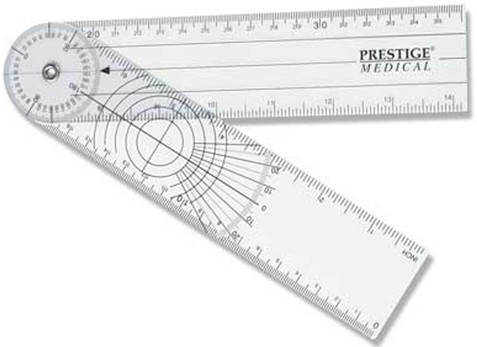
\includegraphics[width=.3\columnwidth]{images/goniometro.png}
	\caption{Goni\'ometro de dos brazos}
	\label{fig:goniometro}
\end{figure}

La elecci\'on del procedimiento quir\'urgico ser\'a determinada por las caracter\'isticas de la fractura u osteotom\'ia; hueso, regi\'on, tipo de trazo, desviaciones  angulares, rotaciones, acortamientos, n\'umero de fragmentos, tama\~no de los fragmentos  y las condiciones de los tejidos blandos.
 
La selecci\'on del implante o dispositivo adecuado para la osteos\'intesis deber\'a incluir el principio biomec\'anico, el abordaje quir\'urgico, el tipo de dispositivo, sus dimensiones, tipo de bloqueo (si lo requiere), dimensiones de los tornillos, orden de colocaci\'on, etc. Para las fracturas diafisiarias en las que esta indicada la fijaci\'on con un clavo intramedular bloqueado, se necesita una planificaci\'on gr\'afica preoperatoria poco detallada. Las variables que hay que determinar son \cite{RUEDI03}: la longitud y el di\'ametro del clavo intramedular, el rimado o no del canal endomedular y el tipo de bloqueo. La osteos\'intesis con placa requiere una planificaci\'on m\'as detallada, los puntos que deben considerarse son: la correcta longitud, alineaci\'on y rotaci\'on del hueso, el tipo y longitud de la placa, el n\'umero de tornillos y su funci\'on espec\'ifica (compresi\'on interfragmentaria o a trav\'es de la placa). Por \'ultimo, es importante destacar que la planificaci\'on preoperatoria de fracturas que comprometen las superficies articulares tiene mayor exigencias que la de fracturas diafisiarias, puesto que requieren una reducci\'on anat\'omica exacta.

En la estrategia quir\'urgica el cirujano ortopedista deber\'a enumerar los pasos a seguir para el procedimiento con el fin de evitar distracciones y para el conocimiento del equipo quir\'urgico. De esta forma dicho equipo estar\'a mejor preparado para resolver los problemas que se puedan presentar. La estrategia quir\'urgica debe estar en el calco de la planificaci\'on preoperatoria, como se observa en la Figura \ref{fig:planificacion_completa}, y debe de contener los siguientes puntos:

\begin{figure}[htb]
	\centering
	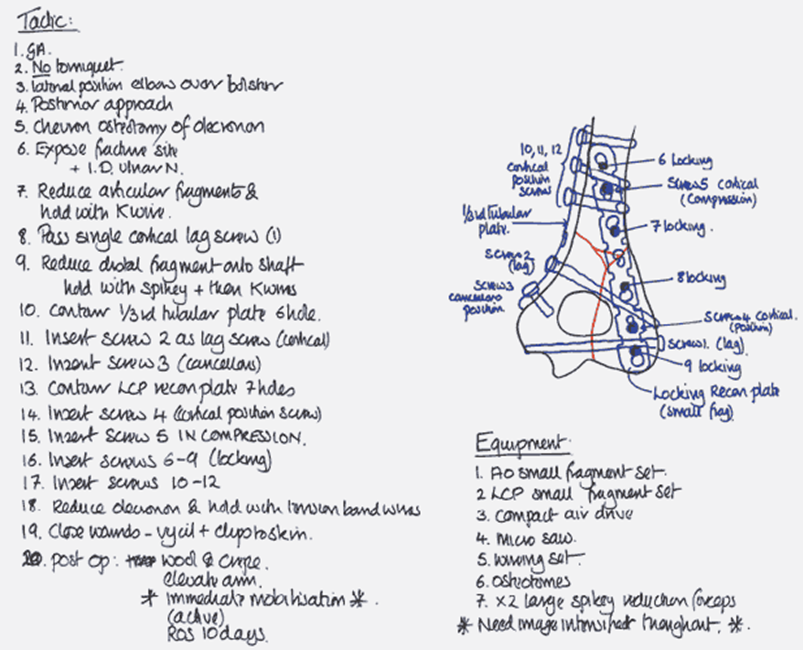
\includegraphics[width=.6\columnwidth]{images/planificacion_completa.png}
	\caption{Calco de una fractura con la informaci\'on completa antes de la cirug\'ia}
	\label{fig:planificacion_completa}
\end{figure}

\begin{itemize}
	\item Paciente: Nombre y apellido, edad, uso de torniquete, posici\'on del paciente, uso de mesa radiol\'ucida.
	\item Procedimiento: Incluye lo referente al abordaje quir\'urgico, principio biomec\'anico, tipo de reducci\'on, implantes a emplear y uso de equipo especial para la colocaci\'on de los mismos.
	\item Equipos Adicionales: Radiograf\'ias transoperatorias, intensificador de im\'agenes, artroscopio, etc.
	\item Cuidados Postoperatorios: Uso de yesos, f\'erulas, pr\'otesis o vendajes en el postoperatorio inmediato.
\end{itemize}


Existen diversas t\'ecnicas de planificaci\'on prequir\'urgica, entre las que se destacan:
\begin{description}
	\item[Superposici\'on directa:] Utilizada en las planificaciones de fracturas diafisiarias. Se realiza el calco de los fragmentos fracturados en una proyecci\'on antero-posterior (AP), cada uno en hojas separadas, en otra hoja se traza una l\'inea recta (eje del hueso) y se coloca los fragmentos que son ensamblados para obtener el resultado final.
	\item[Superposici\'on utilizando la imagen del lado sano:] Se requiere de la radiograf\'ia del lado sano (indirecta) y se procede a realizar el calco del lado fracturado tomando en cuenta los fragmentos y rotaciones dibuj\'andolas en otro color. Luego se realiza la colocaci\'on de los fragmentos dibujados en la radiograf\'ia del lado sano para hacerlos coincidir. Otra forma es realizar la colocaci\'on de los fragmentos y posteriormente superponerla a la radiograf\'ia del lado sano para evaluar la adecuada colocaci\'on de los fragmentos, una vez que se tenga la reducci\'on de los mismos, se utilizan las plantillas de implantes y se completa el calco seg\'un la elecci\'on del cirujano ortopedista.
	\item[Superposici\'on utilizando los ejes fisiol\'ogicos:] Es una metodolog\'ia aplicable a aquellas fracturas periarticulares, como es el caso de las fracturas supracond\'ileas de f\'emur. 
En una fractura distal de f\'emur se usa la plantilla para marcar los ejes anat\'omicos  y mec\'anicos de f\'emur y tibia. Posterior a esto, se dibujan los fragmentos de la fractura y se superponen a la plantilla inicial, para hacer coincidir los ejes del f\'emur, tibia y lograr la alineaci\'on de la rodilla. Una vez colocados todos los fragmentos reducidos se procede a la colocaci\'on del implante.
\end{description}

Particularmente, en este documento trataremos el caso de la planificaci\'on preoperatoria empleando la t\'ecnica de superposici\'on directa.

%%%%%%%%%%%%%%%%%%%%%%%%%%%%%%%%%%%%%%%%%%%%%%%%%%%%%%%%
%%%%%%%%%%%%%%%%%%%%%%%%%%%%%%%%%%%%%%%%%%%%%%%%%%%%%%%%
\section{Sistemas CAD}

El concepto del CAD es amplio y general como herramienta de asistencia a los radi\'ologos, proporcionando una ``segunda opini\'on'' provisto con el computador. Este aspecto \cite{DOI07}, es la principal diferencia con los sistemas de Diagn\'ostico Automatizado por Computador (\textit{Automated Computer Diagnosis}), los cuales son utilizados para diagnosticar cualquier condici\'on de salud-enfermedad (lesi\'on, s\'indrome, entidad nosol\'ogica, etc.). En un sistema CAD siempre el radi\'ologo tomar\'a la decisi\'on final.
 
Las investigaciones en el \'area del Diagn\'ostico Asistido por Computador se iniciaron en el a\~no 1980 y han ido evolucionando gradualmente como una herramienta de apoyo cl\'inico. En el \'area de mamograf\'ia \cite{HUANG07}, los sistemas CAD se han convertido en un procedimiento de rutina para la detecci\'on de c\'anceres de mama en muchos centros m\'edicos. Un gran n\'umero de sistemas CAD en Estados Unidos y Europa \cite{DOI07}, son utilizados para la detecci\'on temprana del c\'ancer de mama en las mamograf\'ias. Algunos sistemas CAD son utilizados para el registro de im\'agenes \cite{ZITO03} (\textit{image registration}), interacciones virtuales, visualizaci\'on, simulaci\'on y entrenamiento.

Por ejemplo, para los casos de entrenamiento y pr\'acticas educativas para estudiantes de medicina, se ofrece una herramienta que simula escenarios virtuales a los futuros cirujanos \cite{BLYT06}. La necesidad de una simulaci\'on viene determinada por la complejidad de ciertas regiones del cuerpo humano, como la craniofacial o la regi\'on card\'iaca. Es muy importante que estructuras vitales del cuerpo humano no sean da\~nadas durante una operaci\'on, lo cual puede lograrse con el uso de sistemas de este tipo.

En el 2002, Bourquain et al. \cite{BOUR02} desarrollaron una aplicaci\'on (\textit{HepaVision2}) para la planificaci\'on preoperatoria para los transplantes y cirug\'ias de h\'igado. \textit{HepaVision2} es una herramienta que trabaja con im\'agenes en formato DICOM \cite{REF_DICOM} (\textit{Digital Imaging and Communication in Medicine}) siendo capaz de realizar una segmentaci\'on del h\'igado empleando el algoritmo \textit{livewire} \cite{MORT95} de detecci\'on de bordes semiautom\'atico. Adem\'as, realiza el c\'alculo del volumen del h\'igado y las venas hep\'aticas que permiten determinar los tumores. Esta versi\'on del software trabaja sobre PC's basadas en \textit{Windows} y provee un m\'odulo de an\'alisis de riesgo de operaci\'on en el paciente a tratar.

%%%%%%%%%%%%%%%%%%%%%%%%%%%%%%%%%%%%%%%
\subsection{CAOS - Cirug\'ia Ortop\'edica Asistida por Computador, \textit{Computer Aided Ort-hopaedic Surgery}}

Diversos softwares de apoyo al cirujano para la reducci\'on de fracturas en extremidades inferiores son utilizados desde hace varios a\~nos \cite{TOCKUS98} \cite{NAKA24}. Los sistemas CAD de planificaci\'on preoperatoria de cirug\'ias del sistema muscoesquel\'etico, son conocidos como CAOS (\textit{Computer Aided Orthopaedic Surgery}) los cuales son foco de investigaci\'on en diversas partes del mundo \cite{BRAN99} \cite{LANG98} \cite{RADE98} \cite{MART00}. Una gran parte de estos sistemas est\'an destinados a garantizar que el cirujano sea capaz de conseguir la posici\'on del implante que ha sido planificado previamente con un sistema CAOS \cite{DIGI98} \cite{OTOO95}. Esto implica que la planificaci\'on preoperatoria conseguida con \'estas herramientas es m\'as precisa y repetible que los m\'etodos convencionales, como el uso de plantillas mostrado en la Figura \ref{fig:plantilla}. Las plantillas son implantes bases construidas por un fabricante bajo diversos materiales y con diferentes medidas, que sirven de gu\'ia exacta en la escogencia de los mismos para una reducci\'on y fijaci\'on interna.

\begin{figure}[htb]
	\centering
	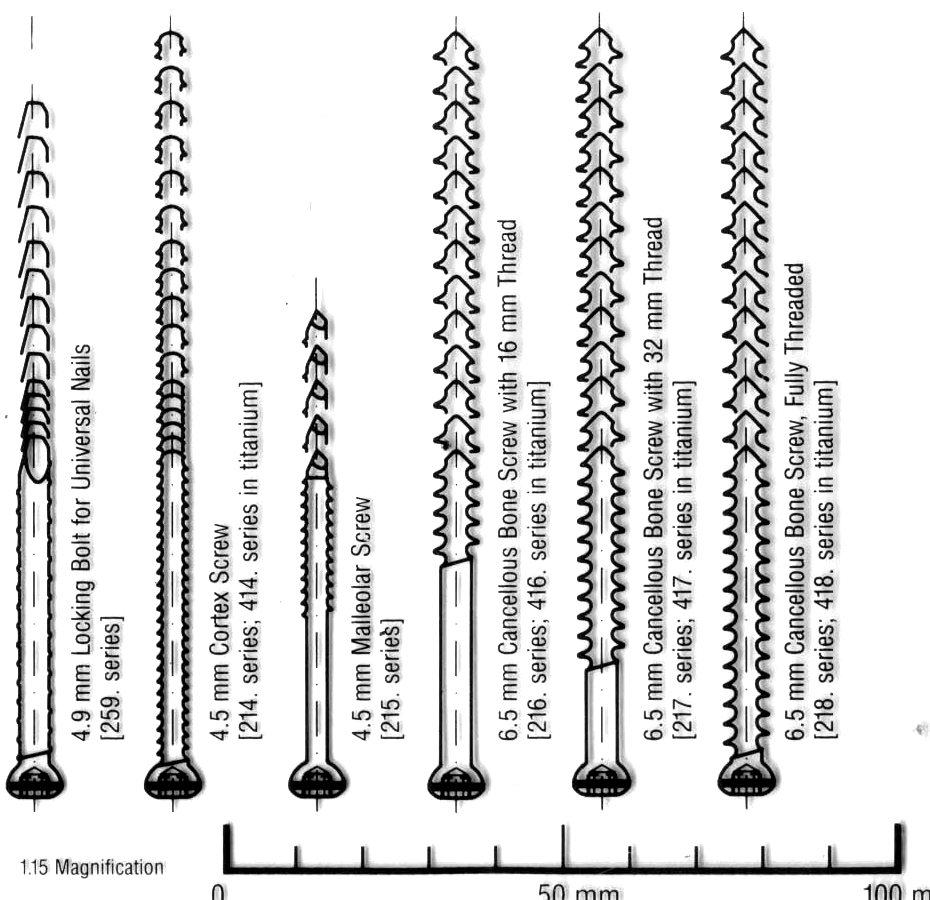
\includegraphics[width=.4\columnwidth]{images/plantillas.png}
	\caption{Plantilla (\textit{template}) de clavos intramedulares}
	\label{fig:plantilla}
\end{figure}

La interpretaci\'on de cualquier imagen m\'edica es un gran problema, ya que no existe un algoritmo trivial el cual puede ser empleado dentro de sistemas automatizados que permita entender la informaci\'on contenida dentro de una imagen. Particularmente, en el \'area de radiolog\'ia, la detecci\'on autom\'atica de fracturas en im\'agenes de Rayos-X (RX) es un problema.

%%%%%%%%%%%%%%%%%%%%%%%%%%%%%%%%%%%%%%%%%%%%%%%%%%%%%%%%
%%%%%%%%%%%%%%%%%%%%%%%%%%%%%%%%%%%%%%%%%%%%%%%%%%%%%%%%
\section{Antecedentes} 

Como vimos anteriormente, la elecci\'on del procedimiento quir\'urgico viene determinado por las caracter\'isticas de la fractura u osteotom\'ia; hueso, regi\'on, tipo de trazo, desviaciones angulares, rotaciones, acortamientos, n\'umero de fragmentos, tama\~no de los fragmentos y las condiciones de los tejidos blandos. Se debe crear un plan para la cirug\'ia que incluya todos los pasos (ordenados) a realizar en el acto quir\'urgico \cite{website:ruedi}. Los sistemas CAD son excelentes herramientas para que los m\'edicos realicen diagn\'osticos m\'as acertados en un tiempo m\'as corto. Cada vez es m\'as frecuente la presencia de estos sistemas en el campo de la medicina, y particularmente existe un gran crecimiento en el \'area de Radiolog\'ia \cite{DOI07}.

La literatura relacionada con sistemas CAD para fracturas es poca; pero existen trabajos relevantes centrados en la detecci\'on de osteoporosis  y estimaci\'on de la edad de huesos. Uno de los trabajos de mayor aporte en el \'area de detecci\'on de fracturas en huesos largos fue el realizado por Tian et al. \cite{TIAN03} en el 2003, los cuales desarrollaron un algoritmo para detectar las fracturas en el f\'emur y el radio. El m\'etodo descrito por Tian \cite{TIAN03} detecta una fractura en el f\'emur al calcular el \'angulo entre el eje del cuello del f\'emur y el eje del f\'emur, llamado \'angulo NSA (\'Angulo del Cervico Diafisiario - textit{Neck-Shaft Angle}), trabajando sobre im\'agenes de CT en formato DICOM. Esta medida del \'angulo es realizada en tres etapas: la primera etapa consiste en la extracci\'on del contorno del f\'emur, ver Figura \ref{fig:tian}, la segunda etapa se refiere al c\'alculo del \'angulo NSA, y la tercera es la clasificaci\'on del \'angulo obtenido. La extracci\'on del contorno del f\'emur descrita por Tian, utiliza la detecci\'on de bordes propuesta por Canny \cite{CANNY86}, la transformada de Hough \cite{DUDA72} y un modelo de Contornos Activos \cite{KASS88}. Las pruebas de este algoritmo mostradas en \cite{YAP04} muestran que detecta una fractura de f\'emur con una precisi\'on del 61.5\%.

\begin{figure}[htb]
	\centering
	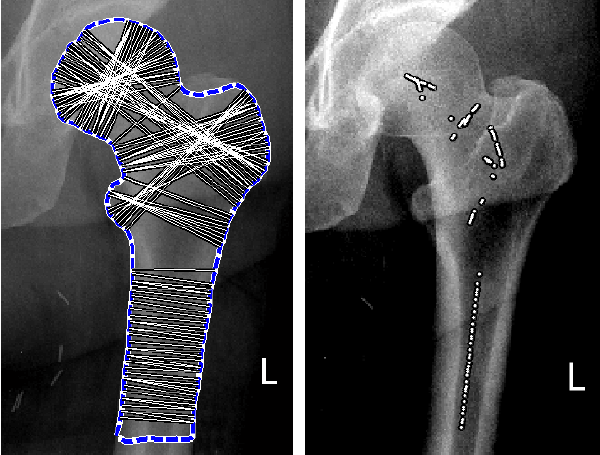
\includegraphics[width=.4\columnwidth]{images/tian.png}
	\caption{L\'ineas encontradas en la detecci\'on del contorno del fem\'ur y l\'ineas gu\'ias para determinar la l\'inea central del fem\'ur}
	\label{fig:tian}
\end{figure}

En el 2004, Yap et al. \cite{YAP04} mejoran el m\'etodo aplicado por Tian, tambi\'en sobre im\'agenes de CT, incluyendo el an\'alisis de la perturbaci\'on de los patrones presentes en la trabecular del cuello femoral. Igualmente, su m\'etodo consiste en 3 etapas: la extracci\'on del contorno del f\'emur, el an\'alisis de la textura trabecular, y la clasificaci\'on de la fractura. Para la extracci\'on del f\'emur en la imagen utilizaron un modelo de Contornos Activo (\textit{snake}) con flujo del vector gradiente. Los resultados obtenidos en este trabajo arrojaron un 84.6\% de exactitud en la detecci\'on de fracturas.

Ambos m\'etodos producen resultados aceptables; pero solo trabaja sobre fracturas localizadas en el cuello femoral y no puede ser adaptada para otros huesos. Tambi\'en requieren una participaci\'on por parte del m\'edico como usuario, ya que debe colocar los puntos iniciales del Contorno Activo y realizarlo la cantidad de veces que sea necesario hasta lograr los resultados esperados.

Una mejora a estos m\'etodos fue introducida por Lim et al. \cite{LIM04} en el 2004, donde se modifica el algoritmo de extracci\'on del contorno propuesto por Tian incluyendo Campos Aleatorios de Markov (\textit{MRF - Markov Random Fields}) e intensidad en la direcci\'on del gradiente (\textit{IGD - Intensity Gradient Direction}) al m\'etodo existente del NSA y mapas de orientaci\'on Gabor (\textit{GO - Gabor Orientation}) \cite{AKDE05}. Adem\'as Lim et al. modificaron la clasificaci\'on planteada en \cite{YAP04}, y consiguieron una detecci\'on de fracturas del 92.2\% de exactitud y 1\% de falsos positivos.

Los m\'etodos explicados anteriormente trabajan con im\'agenes CT en formato DICOM obtenidas directamente desde los equipos radiol\'ogicos. Este aspecto resulta una ventaja ya que la adquisici\'on de las im\'agenes se realiza en un solo paso, empleando la arquitectura existente (e.g. PACS \cite{INCH00} Sistema de Archivo y Transmisi\'on de Im\'agenes - \textit{Picture Archiving and Communication System}) en el centro hospitalario.

Al resultar la segmentaci\'on de huesos un aspecto muy ligado a la anatom\'ia del mismo, existen m\'etodos de clasificaci\'on que eval\'uan las caracter\'isticas de la imagen de una fractura y la ubica en un tipo de fractura. Uno de \'estos es el m\'etodo planteado por Su et al. \cite{SU99} los cuales utilizaron una red neuronal como sistema clasificatorio de fracturas.

Los sistemas CAD de planificaci\'on preoperatoria para fracturas fueron surgiendo como una opci\'on donde la segmentaci\'on autom\'atica de los fragmentos de la fractura, es semi-autom\'atica o manual. En el 2001, Mihalko et al. \cite{MIHA01} presentan un sistema CAD que permite medir la longitud del hueso antes y despu\'es de la colocaci\'on de un implante para as\'i medir la deformaci\'on del mismo, siendo una herramienta preoperatoria y postoperatoria de una fractura.

En el 2002, Viceconti et al. \cite{VICE03} presentan un sistema de planificaci\'on preoperatoria para el reemplazo total de cadera donde se utilizan radiograf\'ias convencionales, lo cual permite ser aplicado a una amplia gama de casos de pacientes de un Centro Hospitalario. Basado en la idea de aplicar planificaci\'on sobre radiograf\'ias convencionales, salieron al mercado sistemas CAOS como NovaRAD \cite{REF_NOVA}, TraumaCAD \cite{REF_TRAUMA} y Sectra OrthoStation Package \cite{REF_SECTRA}, los cuales permiten realizar la planificaci\'on preoperatoria de forma digital y ofrecen una librer\'ia de implantes comerciales a utilizar. 

Estos sistemas CAOS son sumamente costosos y se basan en la existencia de un PACS dentro del Centro Hospitalario, adem\'as de requerir la utilizaci\'on de scanners digitales, tom\'ografos, etc. como mecanismos de adquisici\'on de im\'agenes. Los sistemas CAOS aqu\'i mencionados, \cite{REF_NOVA} \cite{REF_TRAUMA} \cite{REF_SECTRA}, poseen una librer\'ia de implantes donde el m\'edico cirujano selecciona uno de \'estos para ser colocados en la fractura en cuesti\'on, tal como se muestra en la Figura \ref{fig:trauma_cads} (implante en color verde). En muchas ocasiones, es necesario moldear el implante tal que sea anat\'omicamente correcto y se adapte a una secci\'on del cuerpo. Esta deformaci\'on del implante se realiza previo a la operaci\'on, dentro del quir\'ofano, aplicando una fuerza mec\'anica; pero dichos sistemas no lo aplican ya que presentan plantillas no deformables.

\begin{figure}[htb]
	\centering
	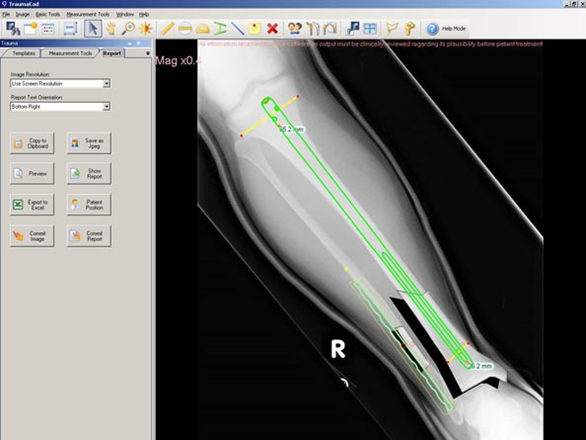
\includegraphics[width=.45\columnwidth]{images/trauma_cads.png}
	\caption{Colocaci\'on de un implante dentro de la aplicaci\'on TraumaCAD de OrthoCrat Ltd.}
	\label{fig:trauma_cads}
\end{figure}

A continuaci\'on se presentar\'a un esquema general para los sistemas CAOS en la realizaci\'on de la planificaci\'on preoperatoria digital, incluyendo funcionalidades adicionales no existentes dentro de los sistemas mencionados anteriormente.

%%%%%%%%%%%%%%%%%%%%%%%%%%%%%%%%%%%%%%%%%%%%%%%%%%%%%%%%
%%%%%%%%%%%%%%%%%%%%%%%%%%%%%%%%%%%%%%%%%%%%%%%%%%%%%%%%
\section{Esquema de planificaci\'on preoperatoria digital}

En la Figura \ref{fig:esquema} se plantea un esquema general para los sistemas de planificaci\'on preoperatoria en el \'area de Traumatolog\'ia. Dicho esquema se puede resumir en ocho grandes m\'odulos constitutivos de la misma. 

\begin{figure}[htb]
	\centering
	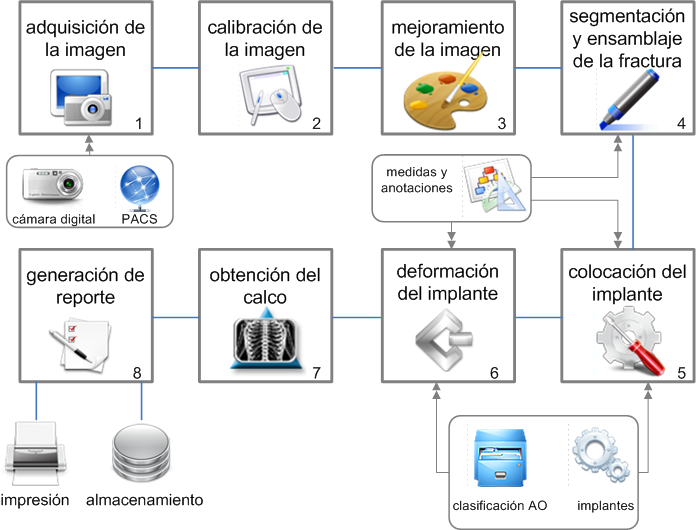
\includegraphics[width=.7\columnwidth]{images/esquema.png}
	\caption{Esquema general de la planificaci\'on preoperatoria digital en Ortopedia}
	\label{fig:esquema}
\end{figure}

El sistema recibe como entrada una imagen correspondiente a una fractura de un paciente, la cual proviene de una placa radiogr\'afica. Una vez adquirida la imagen se procede a un proceso de calibraci\'on, y de esta forma obtener medidas aproximadas de las proporciones dentro de la imagen (e.g. longitud del hueso). A la imagen calibrada se le aplican t\'ecnicas de mejoramiento como aumento del brillo, contraste, etc. que ayuden a realizar la extracci\'on de los fragmentos de una fractura por parte del traumat\'ologo. El traumat\'ologo una vez haya separado los fragmentos de huesos, efect\'ua el ensamblaje del hueso afectado como parte del procedimiento de planificaci\'on.

La fractura tratada puede requerir de un dispositivo externo (placa, tornillo, implante, etc.) para la reducci\'on del hueso, dicho dispositivo ser\'a seleccionado desde un conjunto de templates asociados al tipo de fractura a tratar. Una vez colocado el dispositivo externo, el sistema permite al radio\'logo aplicar deformaciones dependiendo de la anatom\'ia de la reducci\'on. Al finalizar los pasos antes mencionado, se obtiene el calco necesario para la cirug\'ia. La generaci\'on de un reporte con los datos explicados en la Secci\'on \ref{proce} son generados por el sistema, as\'i como el almacenamiento de la planificaci\'on como parte de la historia cl\'inica del paciente.

Cada uno de los pasos de la Figura \ref{fig:esquema} son explicados en detalle a continuaci\'on:

%%%%%%%%%%%%%%%%%%%%%%%%%%%%%%%%%%%%%%%%%%%%%%%%%%%%%%%%
\subsection{Adquisici\'on de la imagen}
La imagen es la base del sistema, y ser\'a el \'area de trabajo sobre la cual el m\'edico traumat\'ologo realizar\'a la planificaci\'on. La imagen ser\'a una radiograf\'ia por ser la modalidad sobre la cual se tratan las fracturas. Para la adquisici\'on de la imagen se plantean dos posibles escenarios:
\begin{enumerate}
	\item Empleando un sistema PACS: obtener la radiograf\'ia de la infraestructura de un PACS. Un PACS posee una integraci\'on \cite{INCH00} de dispositivos de captura de im\'agenes heterog\'eneas, empleando el est\'andar DICOM para el formato de las mismas. El formato DICOM tiene la capacidad de mostrar datos esenciales de los estudios realizados en un paciente (e.g. nombre del paciente, calibraci\'on del equipo empleado, entre otros).
	\item Empleando una c\'amara digital: obtener la radiograf\'ia desde la captura de una placa convencional colocada sobre un equipo de contraste (i.e. negatoscopio, ver Figura \ref{fig:negatoscope}). De esta forma, no es requerido una arquitectura PACS dentro del Centro Hospitalario por ser una t\'ecnica de adquisici\'on de bajo costo. Adicionalmente, permite planificar estudios realizados en equipos convencionales. Los problemas relacionados est\'an vinculados con la calidad de la imagen capturada y la calibraci\'on de la misma.
\end{enumerate}

\begin{figure}[htb]
	\centering
	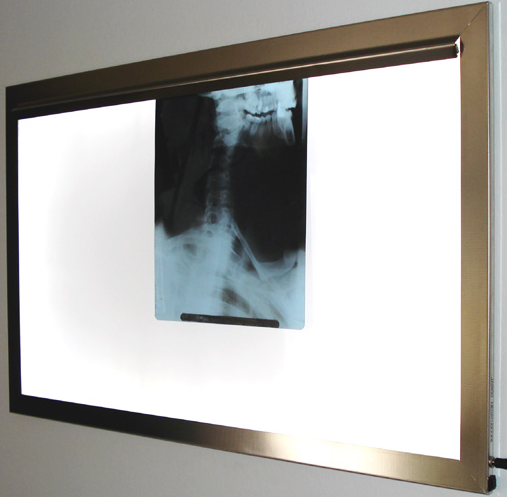
\includegraphics[width=.3\columnwidth]{images/negatoscope.png}
	\caption{Placa radiogr\'afica colocada sobre un negatoscopio}
	\label{fig:negatoscope}
\end{figure}

En ambos escenarios es importante destacar que dichas im\'agenes ser\'an la base para realizar la reconstrucci\'on de las fracturas a trav\'es de los procedimientos traumatol\'ogicos correspondientes.

%%%%%%%%%%%%%%%%%%%%%%%%%%%%%%%%%%%%%%%%%%%%%%%%%%%%%%%%
\subsection{Calibraci\'on de la imagen} \label{CALIB}

Una vez obtenida la imagen del paciente, empieza la fase de calibraci\'on de la imagen la cual permite realizar medidas cuantitativas dentro de la imagen. Estas medidas son siempre aproximadas y generalmente expresadas en mil\'imetros. Para el traumat\'ologo es importante describir la orientaci\'on anat\'omica de la toma; dicha orientaci\'on puede ser antero-posterior o lateral. Al mismo tiempo indicar si la fractura observada se refiere al lado derecho o izquierdo de ciertas partes del cuerpo (e.g. f\'emur, radio, etc.).

Luego de identificada la secci\'on del cuerpo y la orientaci\'on de la toma, el proceso de calibraci\'on requiere de un objeto gu\'ia, el cual debe estar presente en el momento de la adquisici\'on de la imagen. El objeto gu\'ia debe tener una medida conocida, y servir de base para el c\'alculo de las proporciones de la fractura del hueso a estudiar. En la Figura \ref{fig:calibration} se muestra una calibraci\'on realizada empleando una esfera met\'alica de tama\~no conocido (e.g. 24.5 mm de di\'ametro) y de esta forma determinar una proporci\'on dentro de la imagen con respecto a la esfera.

\begin{figure}[htb]
	\centering
	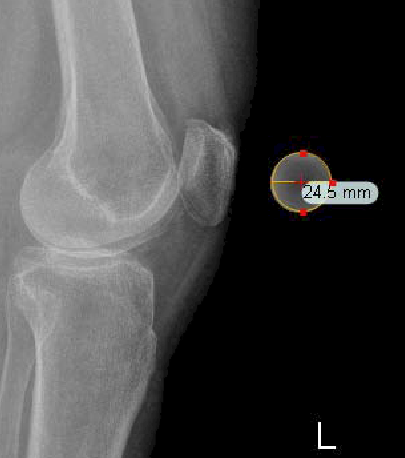
\includegraphics[width=.30\columnwidth]{images/calibration.png}
	\caption{Calibraci\'on empleando una esfera}
	\label{fig:calibration}
\end{figure}

Un aspecto a considerar es el factor de magnificaci\'on \cite{WEBS06}, el cual es inherente en el proceso de toma de los RX. La toma adquirida de un paciente podr\'ia aparecer en mayor proporci\'on que la realidad. El factor de magnificaci\'on depende tanto de la distancia entre el punto focal del tubo de RX y la imagen de la placa, as\'i como la distancia entre el cuerpo que ser\'a sometido al examen y el chasis-pel\'icula, como se observa en la Figura \ref{fig:xray}. Si el paciente se coloca m\'as cercano al punto focal del tubo de RX, el factor de magnificaci\'on es mayor y si se coloca en direcci\'on del chasis-pel\'icula se reduce el factor de magnificaci\'on. Dado que todos los pacientes son diferentes, se crean diferentes factores de aumento en las im\'agenes de RX.

\begin{figure}[htb]
	\centering
		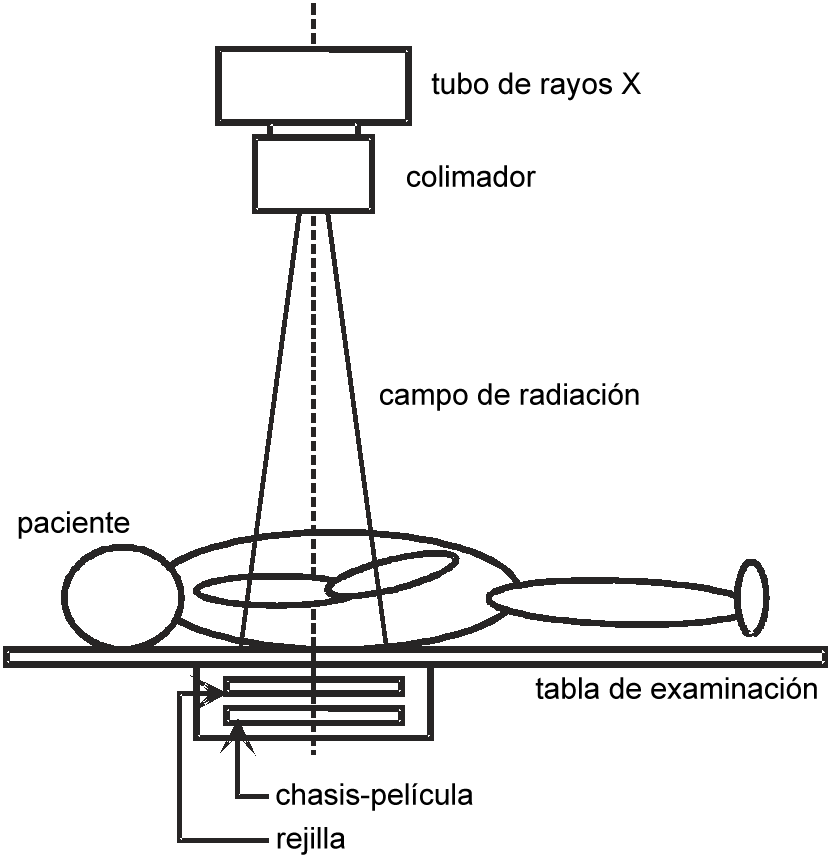
\includegraphics[width=0.40\textwidth]{images/xray.png}
	\caption{Esquema en un examen de Rayos-X}
	\label{fig:xray}
\end{figure}

%%%%%%%%%%%%%%%%%%%%%%%%%%%%%%%%%%%%%%%%%%%%%%%%%%%%%%%%
\subsection{Mejoramiento de la imagen}

Una vez calibrada la imagen, el m\'edico radi\'ologo puede tener la posibilidad de modificar par\'ametros de la imagen que permita mejorar la calidad visual de la misma. Los par\'ametros de calidad que pueden ser modificados son: brillo de la imagen, contraste, invertir los colores, entre otros. Otras operaciones que el traumat\'ologo puede efectuar son:
\begin{itemize}
	\item Cortar la imagen; lo cual permite extraer una imagen de menor dimensi\'on (subimagen) con el objetivo de eliminar de la imagen lo irrelevante para la planificaci\'on.
	\item Rotar la imagen; por las caracter\'isticas de la adquisici\'on de la imagen quiz\'as sea necesario rotarla y obtenerla alineada con respecto a un eje cartesiano, facilitando su manipulaci\'on.
	\item Cambiar el radio aspecto; las proporci\'on entre el ancho y el alto puede ser modificado para ajustar la imagen (aplicando escalamientos), y facilitar la planificaci\'on preoperatoria.
\end{itemize}

%%%%%%%%%%%%%%%%%%%%%%%%%%%%%%%%%%%%%%%%%%%%%%%%%%%%%%%%
\subsection{Segmentaci\'on y ensamblaje de la fractura}

Para efectuar la reducci\'on de una fractura se requiere extraer los fragmentos de hueso presente. Una vez los fragmentos seleccionados, el traumat\'ologo debe ensamblarlos y colocarlos en sus posiciones correctas y completar la reducci\'on de la fractura.

La selecci\'on de los fragmentos de la fractura en la imagen, requiere un proceso de segmentaci\'on \cite{UMB05} donde se separen dichos fragmentos del hueso a tratar. Los algoritmos existentes para la segmentaci\'on autom\'atica de im\'agenes de RX no son triviales ya que no existe un procedimiento est\'andar para su ejecuci\'on. En la literatura existen diversas t\'ecnicas para la segmentaci\'on de im\'agenes m\'edicas \cite{HARA85} \cite{PAL93} \cite{PHAM98} entre las que destacan: los modelos deformables \cite{KASS88} \cite{TER87} \cite{TER88}, las plantillas deformables param\'etricas \cite{YUI92}, los modelos de distribuci\'on de puntos \cite{COOT99} \cite{COOT94}, las plantillas gr\'aficas \cite{AMIT96}, las plantillas basadas en esqueletos \cite{PIZ98} \cite{PIZ99}, entre otras t\'ecnicas. Dichas t\'ecnicas no son 100\% efectivas para todas las im\'agenes. Para conseguir una segmentaci\'on adecuada por lo general se emplean varias de \'estas t\'ecnicas y/o se aplican modificaciones acorde a la imagen en cuesti\'on.

Otra forma de extracci\'on de fragmentos es emplear la segmentaci\'on manual, la cual consiste en delinear los bordes de los fragmentos e ir construyendo un pol\'igono que encierre el fragmento de hueso, como se observa en la Figura \ref{fig:fragment}.

\begin{figure}[htb]
	\centering
		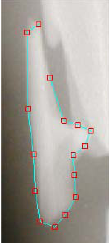
\includegraphics[width=0.15\textwidth]{images/fragment.png}
	\caption{Fragmento de hueso de una fractura extra\'ido manualmente}
	\label{fig:fragment}
\end{figure}

Se observa una serie de puntos gu\'ia (en color rojo) sobre el contorno del fragmento unidos por una l\'inea formando un pol\'igono irregular. El pr\'oximo paso es colocar dicho fragmento en su posici\'on anat\'omicamente correcta para realizar la reducci\'on por parte del radi\'ologo.

%%%%%%%%%%%%%%%%%%%%%%%%%%%%%%%%%%%%%%%%%%%%%%%%%%%%%%%%
\subsubsection{Medidas y anotaciones}

Una vez calibrada la imagen, ver Secci\'on \ref{CALIB}, es posible realizar mediciones de la anatom\'ia en una la imagen empleando diversas herramientas. Las mediciones dentro de una imagen de RX son importantes para el tratamiento de un paciente, ya que permite obtener las dimensiones de los segmentos de una fractura, la longitud de los huesos, un \'angulo entre dos secciones (e.g. huesos de la cadera), entre otros. Generalmente las medidas realizadas son en mm. o en la escala definida en la etapa de calibraci\'on.

Algunas de las herramientas de calibraci\'on se observan en la Figura \ref{fig:medidas} y se explican a continuaci\'on: 

\begin{figure}[htb]
	\centering
	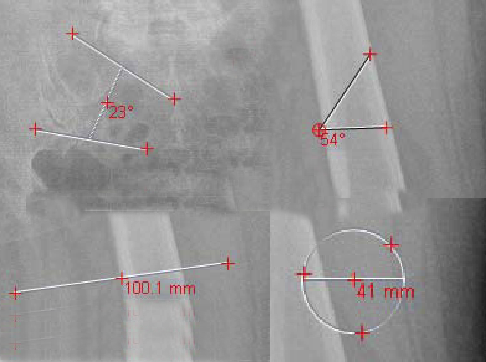
\includegraphics[width=.5\columnwidth]{images/medidas.png}
	\caption{Medidas realizadas en la imagen: inter-l\'inea, \'angulo, regla, c\'irculo}
	\label{fig:medidas}
\end{figure}

\begin{description}
	\item[Inter-l\'inea:] Permite medir el \'angulo existente entre dos l\'ineas en una imagen. Esta herramienta es muy \'util cuando se est\'a trabajando con \'angulos peque\~nos dentro de la imagen
	\item[\'Angulo:] Permite medir \'angulo dentro de la imagen, basado en un punto origen y dos l\'ineas que parten desde ese origen
	\item[Regla:] Con esta herramienta se puede medir regiones de la imagen empleando una l\'inea para dicha labor
	\item[C\'irculo:] Permite realizar un c\'irculo definido por un centro y un di\'ametro, la medida indicada por la misma viene dada por el valor del di\'ametro
\end{description}

Si la imagen no se encuentra calibrada, el valor de la medida realizada ser\'a en p\'ixeles.

Una funcionalidad sumamente \'util dentro de la planificaci\'on de una operaci\'on son las anotaciones. Las anotaciones permite colocar informaci\'on de inter\'es dentro de la imagen (placa RX) en formato de texto. Las notas colocadas dentro de la planificaci\'on son libres a juicio del m\'edico radi\'ologo.

%%%%%%%%%%%%%%%%%%%%%%%%%%%%%%%%%%%%%%%%%%%%%%%%%%%%%%%%
\subsection{Colocaci\'on del implante} \label{IMPLANTE}

Al tener ya los segmentos de hueso de la fractura seleccionados y haber aplicado la reducci\'on de la misma, queda a decisi\'on del traumat\'ologo la colocaci\'on de implantes (\textit{template}) para realizar una fijaci\'on del hueso como parte del tratamiento quir\'urgico. Dependiendo del tipo de fractura (ver Secci\'on \ref{AO}), posici\'on anat\'omica, edad del paciente, entre otros, se procede a seleccionar el adecuado de una librer\'ia de implantes (ver Secci\'on \ref{BIB_IMPL}).

Un hueso fracturado debe ser cuidadosamente colocado (fijaci\'on) en la posici\'on adecuada hasta que sea lo suficientemente fuerte como para soportar el peso. Hasta el siglo pasado \cite{REF_AO}, los m\'edicos se basaron en emplear solamente yesos y f\'erulas para apoyar el hueso por fuera del cuerpo (fijaci\'on externa). Pero el desarrollo en el campo de la cirug\'ia redujo el riesgo de infecci\'on, permitiendo que los m\'edicos puedan trabajar directamente con el hueso y colocar implantes (fijaci\'on interna). 

Nuevos materiales tales como acero inoxidable, cobalto y titanio no son solo duraderos, sino que tambi\'en lo suficientemente fuertes y flexibles para apoyar el hueso. Estos materiales tambi\'en son compatibles con el cuerpo y rara vez causan una reacci\'on al\'ergica en el paciente. Los tipos m\'as comunes de la fijaci\'on son: los alambres, placas, barras, clavijas, pines, clavos y tornillos. 

%%%%%%%%%%%%%%%%%%%%%%%%%%%%%%%%%%%%%%%%%%%%%%%%%%%%%%%%
\subsection{Deformaci\'on del implante}\label{DEFO}

Como vimos anteriormente, los sistemas CAOS deben proveer una librer\'ia de implantes donde el m\'edico cirujano seleccione uno de \'estos para ser colocados en la fractura en cuesti\'on. En muchas ocasiones, es necesario moldear (deformar) el implante tal que sea anat\'omicamente correcto y se adapte a una secci\'on del cuerpo, particularmente al hueso fracturado. Esta deformaci\'on del implante se realiza previo a la operaci\'on aplicando una fuerza mec\'anica.

Partiendo del hecho que el implante es una imagen digital, Beier y Neely \cite{BEIER92} propusieron una t\'ecnica para la metamorfosis de una imagen digital a otra basada en vectores caracter\'isticos. Esta t\'ecnica fue empleada para efectos visuales de transiciones en animaciones; pero es extensible para cualquier prop\'osito de deformaci\'on de im\'agenes.  

En el 2003, Birkholz y Jack\`el \cite{BIRK03} presentan una soluci\'on para la deformaci\'on (\textit{warping}) de im\'agenes digitales, bas\'andose en el trabajo de Beier y Neely pero empleando curvas para la manipulaci\'on y gu\'ia del \textit{warping}. En dicho trabajo se presenta una forma natural de hacer deformaciones sobre las im\'agenes, como se muestra en la Figura \ref{fig:jackel}.

\begin{figure}[htb]
	\centering
		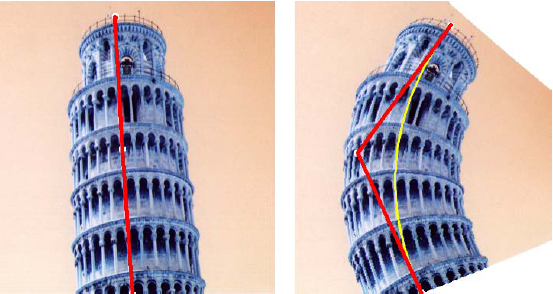
\includegraphics[width=0.60\textwidth]{images/jackel.png}
	\caption{\textit{Warping} desarrollado por Birkholz y Jack\`el \cite{BIRK03}}
	\label{fig:jackel}
\end{figure}

Sobre la imagen se identifican los puntos de control de la curva tal como se muestra en la Figura \ref{fig:jackel}, formando la l\'inea de color rojo. Dichos puntos de control son modificados por el usuario para construir la curva en color amarillo. Esta curva representa la gu\'ia para la deformaci\'on de la imagen en cuesti\'on. De esta forma, tomando los implantes como una imagen digital, es posible efectuar una deformaci\'on de los mismos.

%%%%%%%%%%%%%%%%%%%%%%%%%%%%%%%%%%%%%%%%%%%%%%%%%%%%%%%%
\subsubsection{Biblioteca de clasificaci\'on AO$^2$}\label{AO}

Una vez confirmada la fractura de un paciente es localizada y clasificada de acuerdo a un esquema establecido. El esquema de clasificaci\'on de una fractura est\'a especificada de acuerdo a su ubicaci\'on anat\'omica. Algunas de las m\'as com\'unes son: La clasificaci\'on AO$^2$ \cite{REF_AO}, la clasificaci\'on Salter-Harris \cite{SALT63} y la clasificaci\'on de fracturas abiertas de Gustilo \cite{GUST76}.

En el esquema internacional de clasificaci\'on de fracturas AO$^2$, el m\'edico traumat\'ologo clasifica una fractura de acuerdo a la ubicaci\'on de la misma y sus caracter\'isticas morfol\'ogicas. AO$^2$ plantea una clasificaci\'on basada en dos n\'umeros: el primero indica una ubicaci\'on en el cuerpo (1-h\'umero, 2-c\'ubito y radio, 3-f\'emur y 4-tibia y peron\'e) y el segundo, el segmento dentro del hueso (1-proximal, 2-diafisal, 3-distal). Una vez seleccionado ambos n\'umeros, entra en una clasificaci\'on por tipo de fractura (A-simple, B-en cu\~na, C-compleja). Luego, la fractura es dividida en tres grupos que miden la escala de severidad de la misma (1,2,3). En la Figura \ref{fig:ao_femur} se muestra la clasificaci\'on AO$^2$ para el f\'emur en segmento diafisial.

\begin{figure}[htb]
	\centering
		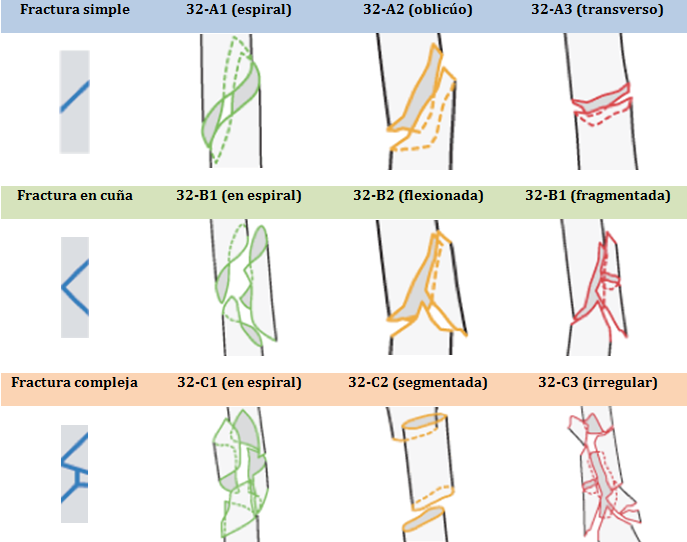
\includegraphics[width=0.60\textwidth]{images/ao_femur.png}
	\caption{Clasificaci\'on AO$^2$ para una fractura tipo 32}
	\label{fig:ao_femur}
\end{figure}

Esta clasificaci\'on es utilizada como una gu\'ia para el pron\'ostico y eficiencia en el tratamiento de una fractura. El esquema AO$^2$ es recomendado internacionalmente porque es cl\'inicamente relevante, sencillo, reproducible y provee una buena estimaci\'on del resultado cl\'inico \cite{MULL98}. Tener una biblioteca de referencia de dicha clasificaci\'on ayudar\'a considerablemente al m\'edico radi\'ologo para que en cualquier momento pueda consultarla para una determinada fractura. En los pasos de Colocaci\'on del implante (Secci\'on \ref{IMPLANTE}) y Deformaci\'on del implante (Secci\'on \ref{DEFO}) es posible acceder a una biblioteca de clasificaci\'on AO$^2$ y a una librer\'ia de implantes.

%%%%%%%%%%%%%%%%%%%%%%%%%%%%%%%%%%%%%%%%%%%%%%%%%%%%%%%%
\subsubsection{Librer\'ia de implantes} \label{BIB_IMPL}

Una librer\'ia de implantes es un conjunto de plantillas (\textit{templates}, ver Figura \ref{fig:plantilla}) de traumatolog\'ia clasificadas bajo alg\'un criterio. De esta forma, se escoge el tipo de implante (e.g. clavo, placa, etc.), las dimensiones (e.g. 12mm, 3.5 mm, etc.), el fabricante y el material. El proceso de seleccionar un implante (ver Secci\'on \ref{IMPLANTE}) de la librer\'ia es un proceso sencillo que depende del m\'edico traumat\'ologo. La decisi\'on sobre cual implante colocar para una fractura tal que se obtenga una cirug\'ia efectiva, es arbitraje del m\'edico.

La librer\'ia de implantes es un conjunto de im\'agenes organizadas bajo cierta estructura que permitan su r\'apido acceso. Una base de datos es una forma de almacenamiento recomendada para colocar la gran cantidad de implantes requeridos para los sistemas CAOS de planificaci\'on preoperatoria. 

%%%%%%%%%%%%%%%%%%%%%%%%%%%%%%%%%%%%%%%%%%%%%%%%%%%%%%%%
\subsection{Obtenci\'on del calco}\label{CALCO}

Al realizar el proceso de colocaci\'on de los implantes requeridos para un paciente, se obtiene una imagen que muestra la fractura en cuesti\'on, los implantes, anotaciones y medidas. Esta imagen es esencial para la generaci\'on del reporte a generar, ver Secci\'on \ref{REPOR}, ya que constituye la base de la misma. 

El calco generado, debe mostrar claramente la posici\'on del implante ya que esta es una gu\'ia para una cirug\'ia. En la Figura \ref{fig:calco} se muestra un calco donde el color de fondo correspondiente a unos RX es blanco. El prop\'osito es obtener un formato de impresi\'on adecuado cuando se vaya a hacer la generaci\'on del reporte. Una vez generado el reporte, ya se encuentra en formato digital permitiendo su impresi\'on, envio por e-mail, almacenamiento en el sistema PACS, etc.

\begin{figure}[htb]
	\centering
		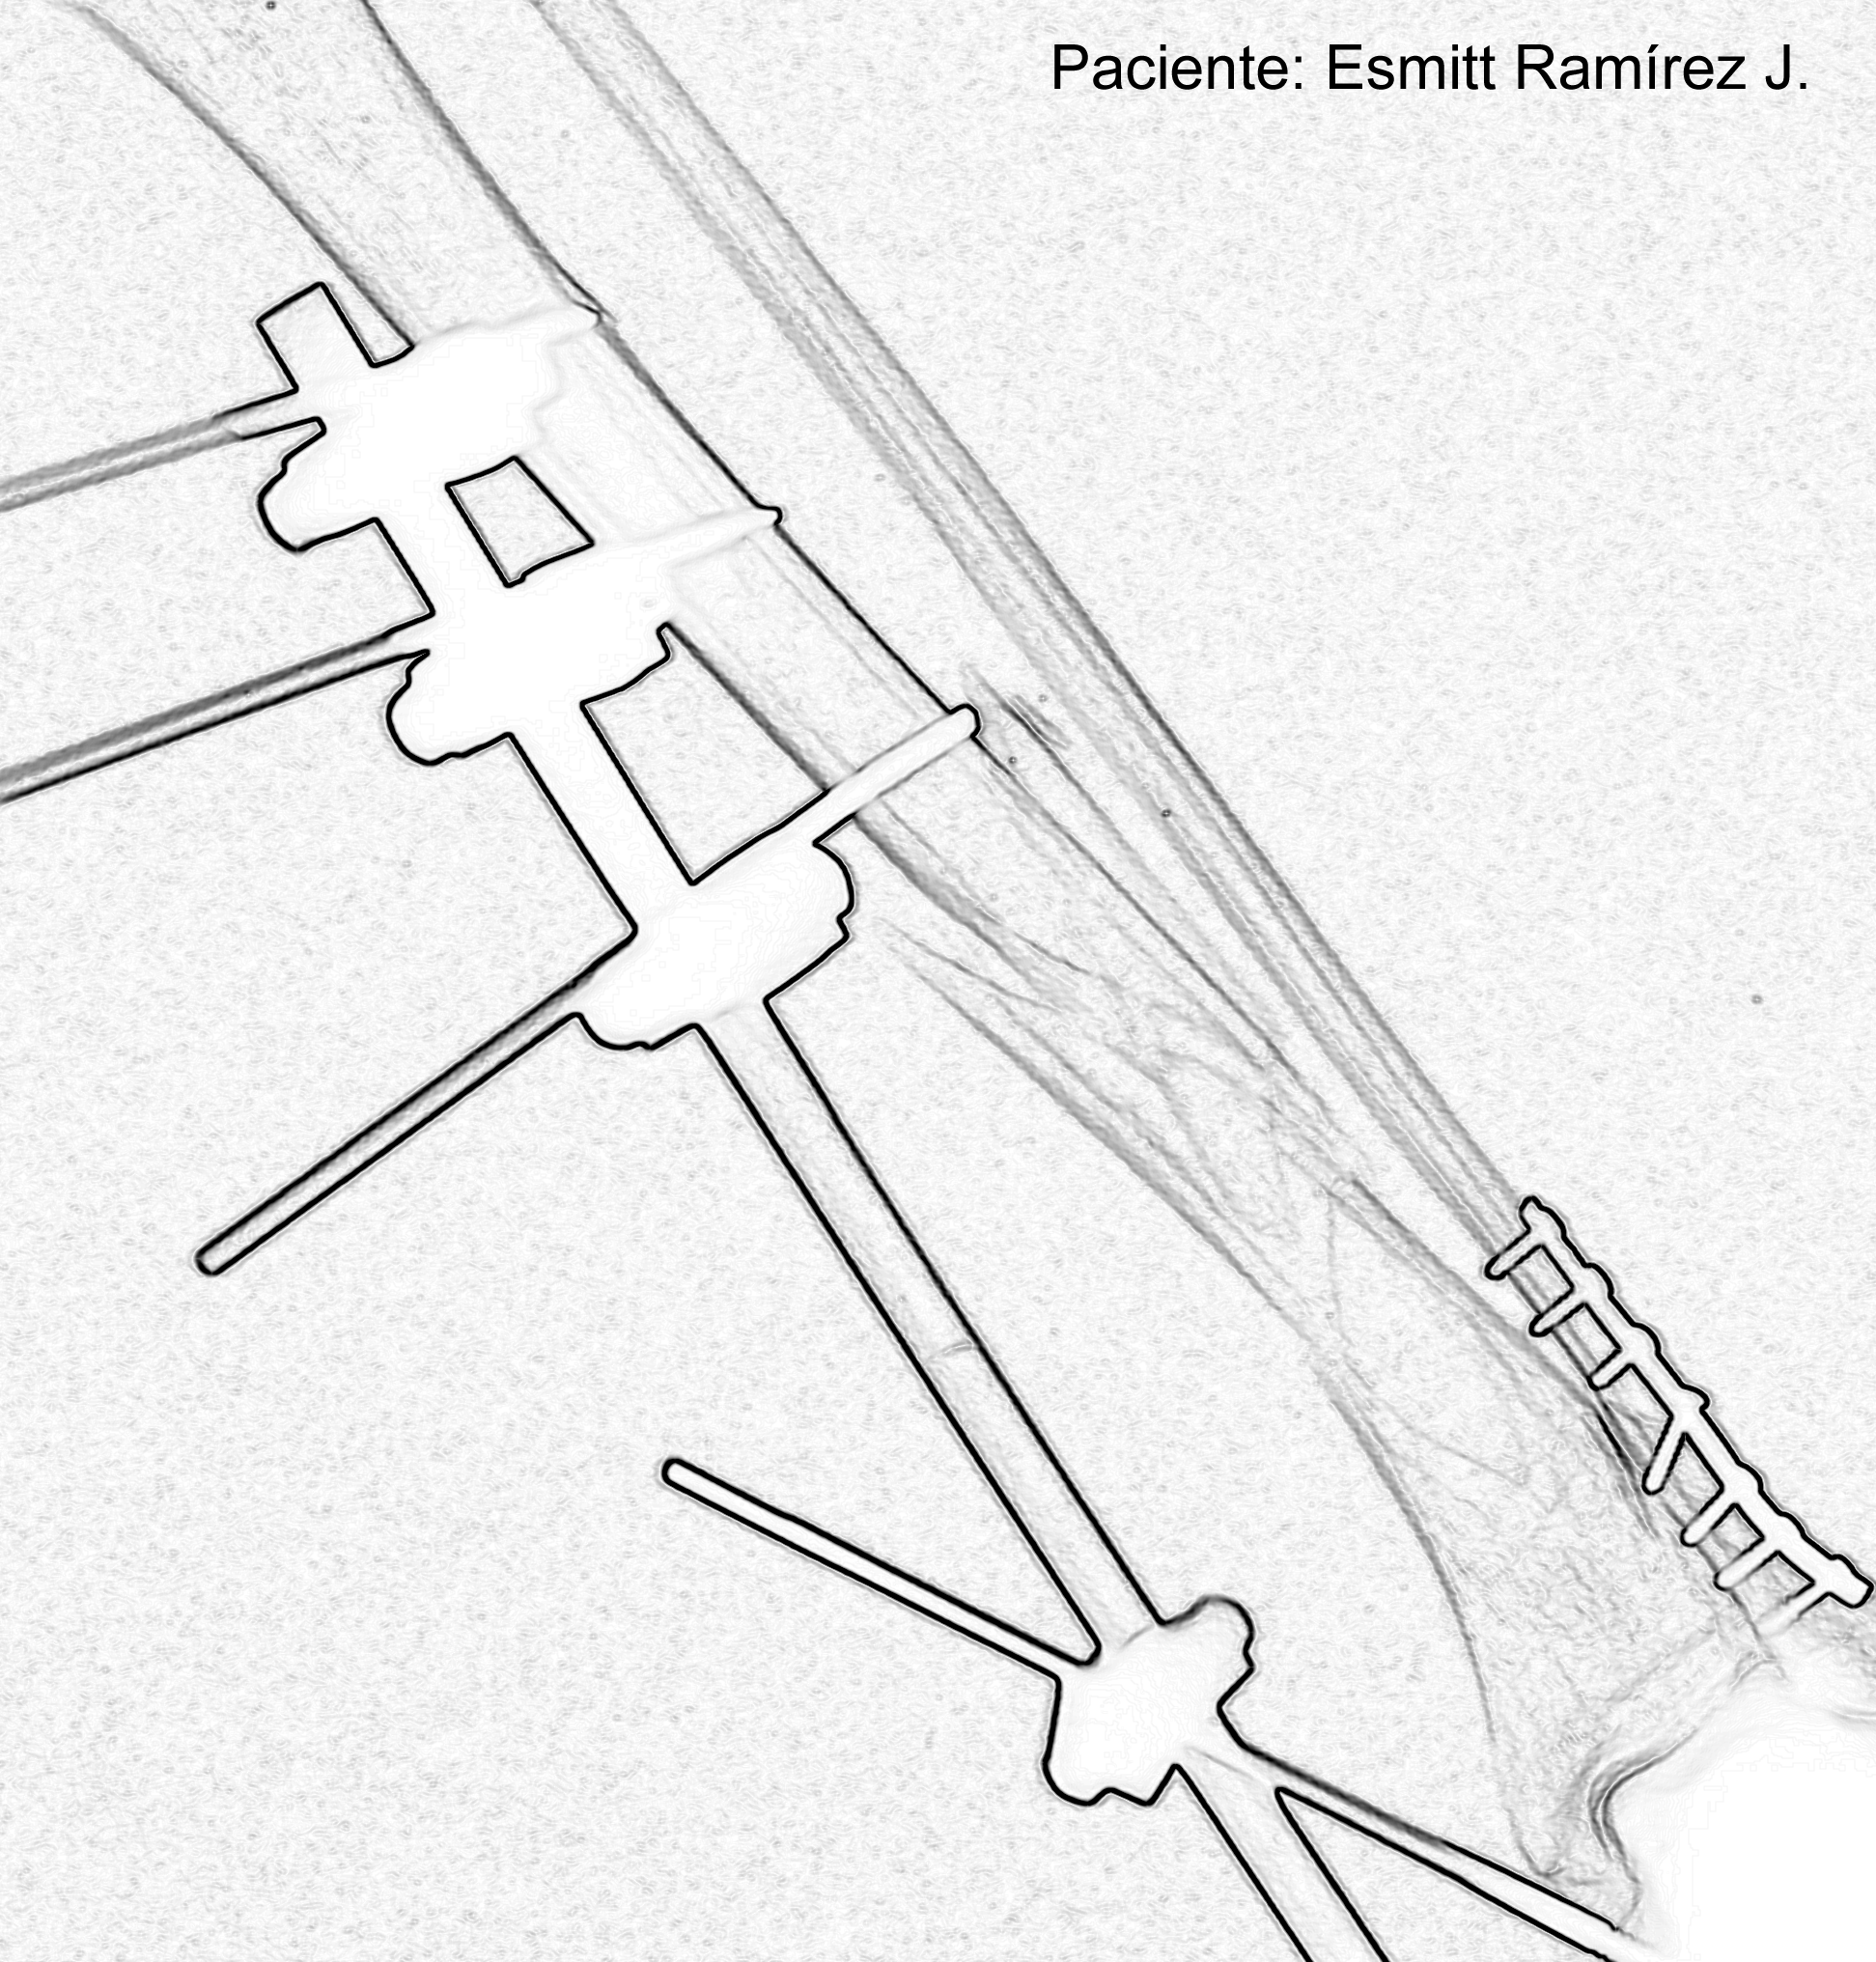
\includegraphics[width=0.35\textwidth]{images/calco.png}
	\caption{Calco en formato de impresi\'on}
	\label{fig:calco}
\end{figure}

%%%%%%%%%%%%%%%%%%%%%%%%%%%%%%%%%%%%%%%%%%%%%%%%%%%%%%%%
\subsection{Generaci\'on de reporte} \label{REPOR}

Un reporte consiste de una imagen seleccionada que incluye implantes, medidas e informaci\'on que describe al paciente, los procedimientos quir\'urgicos que ayudar\'an al m\'edico cirujano en la cirug\'ia. El texto que aparece en un reporte, se encuentra por encima de la imagen o en una caja de texto (\textit{textbox}), y los implantes a utilizar se deben mostrar claramente.

La creaci\'on de un reporte de la planificaci\'on permitir\'a tener un resumen de todo el trabajo realizado en el sistema CAOS de planificaci\'on preoperatoria. Los reportes contribuyen a desarrollar la Telemedicina \cite{MEH02}, la cual consiste en la prestaci\'on de servicios de medicina a distancia, particularmente para el diagn\'ostico.

%%%%%%%%%%%%%%%%%%%%%%%%%%%%%%%%%%%%%%%%%%%%%%%%%%%%%%%%
%%%%%%%%%%%%%%%%%%%%%%%%%%%%%%%%%%%%%%%%%%%%%%%%%%%%%%%%
\section{Conclusiones} Planificar los pasos antes de una cirug\'ia es de vital importancia para garantizar la eficacia de los procedimientos quir\'urgicos en el quir\'ofano. Los pasos a ejecutar para su realizaci\'on son un trabajo extra lo cual implica inversi\'on de tiempo de parte del m\'edico. La existencia de sistemas CAOS de planificaci\'on preoperatoria permiten reducir considerablemente ese tiempo, adem\'as de proveer todas las ventajas que proporciona tener esa informaci\'on en formato digital. El esquema presentado aqu\'i permite tener una estructura s\'olida en el dise\~no de estos sistemas. Los procesos de calibraci\'on, siempre ser\'an aproximaciones (al realizar las mediciones posteriores) ya que al trabajar con im\'agenes digitales, aunado al proceso de adquisici\'on de la imagen, existe una p\'erdida de informaci\'on. La inclusi\'on de la librer\'ia de implantes y su deformaci\'on permite simular el procedimiento dentro del quir\'ofano realizado por el cirujano y su equipo. Adicionalmente, proveer una biblioteca de clasificaci\'on de fracturas (e.g. AO$^2$) permite tener disponible una gu\'ia de referencia en todo momento. A medida que existan nuevos requerimientos en el \'area m\'edica, seguir\'an surgiendo aplicaciones que faciliten y contribuyan a mejores diagn\'osticos as\'i como inversi\'on en costos, tanto como al paciente y al m\'edico.

%%\bibliographystyle{siam}
%%\bibliographystyle{abbrv}
%\bibliographystyle{plain}
\bibliographystyle{babplain}
%%\bibliographystyle{IEEEtran}
%%\bibliographystyle{asr}
%%
\selectbiblanguage{spanish}
%\bibliography{Paper_Siacg}

\bibliography{books}



\end{document}
